%!TEX root = ../Thesis.tex

\chapter{Clusteranalyse von Fahrzeugtrajektorien}
\label{cha:realisation_clustering}

In diesem Kapitel wird die Umsetzung der Clusteranalyse der Trajektorien vorgestellt.
Es wird zuerst darauf eingegangen, welche Trajektorie-Repräsentation gewählt wurde. Anschließend
werden die verschiedenen Schritte zur Bereinigung und Vorverarbeitung der Daten beschrieben, welche
in dieser Arbeit zum Einsatz kommen. Schlussendlich folgt die Erläuterung der eigentlichen Clusteranalyse.
Hier werden die verschiedenen untersuchten Ansätze vorgestellt und ihre Ergebnisse diskutiert.

Die \textit{TrackerApplication} ist in Java und Scala implementiert. Ihre Benutzeroberfläche basiert
auf JavaFX. Das in dieser Arbeit erstellte Modul \textit{Spurerkennung} wird komplett mit Scala umgesetzt. 

\section{Trajektorie-Definition}

Die Ergebnisse der Fahrzeugverfolgung (siehe Abschnitt \ref{sec:position_extraction}) werden
in der \textit{TrackingApplication} in Form sogenannter \textit{TrackedObject}`s gespeichert.
Ein solches Objekt repräsentiert eine zusammenhängende, nicht unterbrochene Verfolgung eines Fahrzeugs.
Wird eine Verfolgung, beispielsweise aufgrund einer Überdeckungen, unterbrochen, so existieren für ein
Kraftfahrzeug mehrere Objekte, welche sich einander nicht zuordnen lassen.
Die wichtigsten Informationen, die ein \textit{TrackedObject} beinhaltet, sind eine eindeutige ID,
die Frame-Positionen des Starts und Endes der Verfolgung und die Objekt-Klasse des Fahrzeugs. Es wird
zwischen den vier Klassen \textit{``Auto''}, \textit{``Lastwagen''}, \textit{``Transporter''}
und \textit{``Zweirad''} unterschieden.
Für jedes verfolgte Objekt können die zugehörigen Positions-, Geschwindigkeits-, Beschleunigungs-
und Dimensions-Informationen abgerufen werden. Diese werden für jedes Frame, welches zwischen dem Start-
und End-Frame des Objektes liegt, bestimmt.

Da für die Ableitung von Fahrspuren aus Trajektorien lediglich die positionsbezogenen Eigenschaften
der Fahrzeuge relevant sind, werden Bewegungbahnen in dieser Arbeit über jene definiert.
Geschwindigkeit, Beschleunigung und Dimension der Fahrzeuge wird in der Clusteranalyse nicht berücksichtigt.
Abbildung \ref{fig:real_trajectory_classDia} zeigt den Aufbau einer Trajektorie im Modul \textit{Spurerkennung}.

\begin{figure}[H]
\centering
    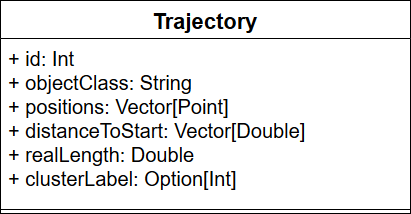
\includegraphics[width=0.38\linewidth]{../resources/img/umsetzung/U1/Trajectory_ClassDia}
\caption{Aufbau Trajektorie-Klasse}
\label{fig:real_trajectory_classDia}
\end{figure}

Die Felder \textit{id} und \textit{objectClass} werden aus dem der Trajektorie zugrundeliegenden \textit{TrackedObject}
übernommen. 
Die Positionen eines Fahrzeugs werden in Form von 2D-Welt-Koordinaten (siehe Abschnitt \ref{sec:position_extraction})
in \textit{positions} gespeichert und die Anzahl der Koordinaten zusätzlich in \textit{pointLength}.
Die Sequenz \textit{distToStart} enthält für jeden Punkt der Bewegungsbahn die Distanz zum Start der Trajektorie in Metern.
Die Werte ergeben sich aus Formel \ref{eq_real_distToStart}, wobei $p_n$ dem $n$-ten Punkt in der Trajektorie entspricht
und $dist$ der euklidschen Distanz zwischen zwei Punkten.

\begin{ceqn}
\begin{align}
\label{eq_real_distToStart}
    distToStart(p_n) =
    \begin{cases}
        0 & \text{if } n = 0 \\
        dist(p_n,\ p_{n-1}) + distToStart(p_{n-1}) & \text{otherwise} 
    \end{cases}
\end{align}
\end{ceqn}

Aus \textit{distToStart} ergibt sich zudem die Gesamtlänge einer Trajektorie, welche extra gespeichert wird.
Das Feld \textit{clusterLabel} ordnet jede Trajektorie nach der Clusteranalyse einem bestimmten Cluster zu.
Zuvor enthält es keinen Wert.

% TODO: Evtl Bilder und Beschreibung austauschen
Zur Untersuchung der Fahrzeugtrajektorien ist es hilfreich diese zu visualisieren. Abbildung \ref{fig:real_trajs_raw_neckartor}
zeigt so beispielsweise 1240 Trajektorien, welche aus einer Aufnahme des Stuttgarter Neckartors extrahiert wurden.
In Abbildung \ref{fig:real_neckartor} ist ein Ausschnitt der entsprechenden Aufnahme zu sehen.

\begin{figure}[H]
\centering
    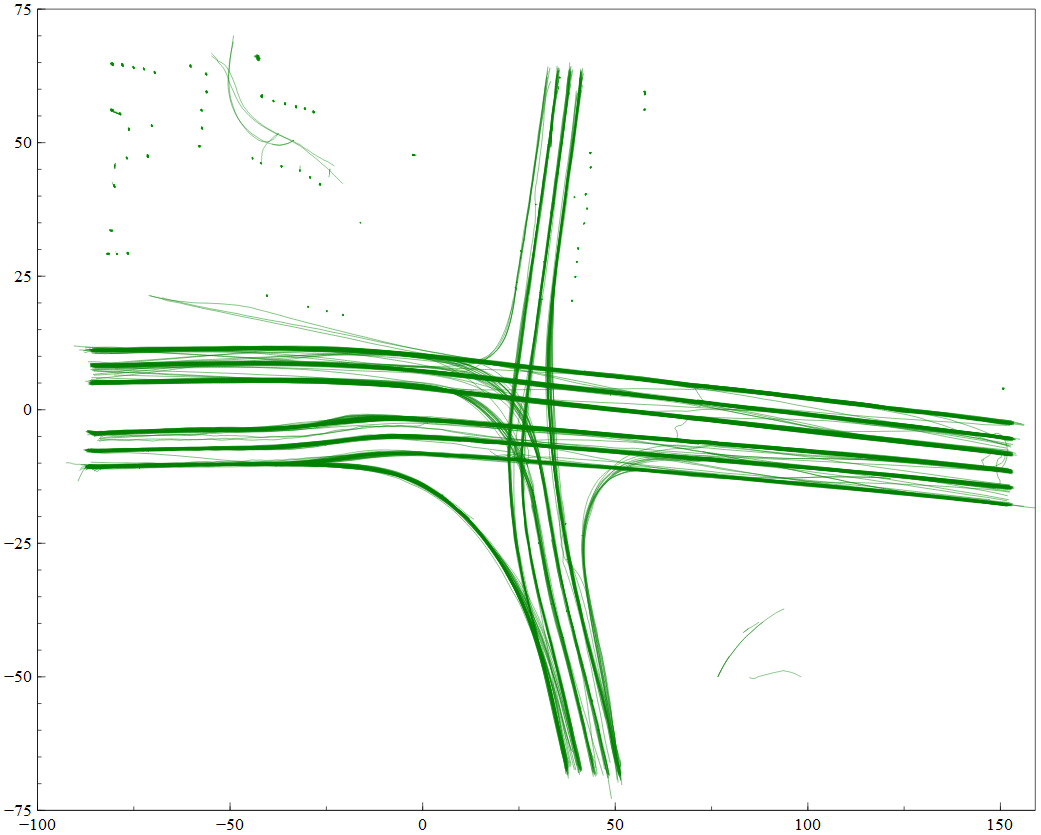
\includegraphics[width=0.5\linewidth]{../resources/img/umsetzung/U1/Plot_RawTrajectories_Neckartor}
\caption{Unverarbeitete Trajektorien vom Stuttgarter Neckartor}
\label{fig:real_trajs_raw_neckartor}
\end{figure}

\begin{figure}[H]
\centering
    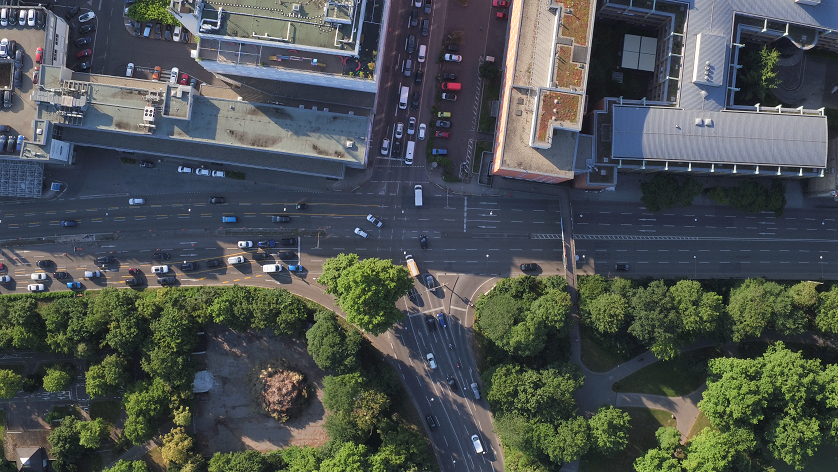
\includegraphics[width=0.7\linewidth]{../resources/img/umsetzung/U1/Neckartor_Aufnahme}
\caption{Das Stuttgarter Neckartor}
\label{fig:real_neckartor}
\end{figure}

In Abbildung \ref{fig:real_trajs_raw_neckartor} sind die verschiedenen Bewegungsbahnen der Fahrzeuge für
den menschlichen Betrachter bereits klar erkennbar.
Direkt fallen aber auch die Trajektorien der stehenden oder sich auf Parkplätzen
bewegenden Autos im oberen Bereich der Aufnahme ins Auge. Diese dürfen nicht in die Clusteranalyse mit einbezogen werden.
Bei genauerer Untersuchung der Trajektorien zeigen sich weitere Probleme, welche das Clustering negativ
beeinflussen würden. Zwei sind in nachfolgender Abbildung dargestellt.
\ref{fig:real_defects_trajectories} a) zeigt, wie Fahrzeuge Punktwolken beim Stilstand vor Lichtsignalanlagen bilden.
In \ref{fig:real_defects_trajectories} b) wird deutlich, dass in manchen Bereichen sehr viele Trajektorie-Unterbrechungen
auftreten. Hier wird die Straße üblicherweise von Bäumen, Brücken et cetera überlagert.

\begin{figure}[H]
    \centering
    \subfloat[]{{
        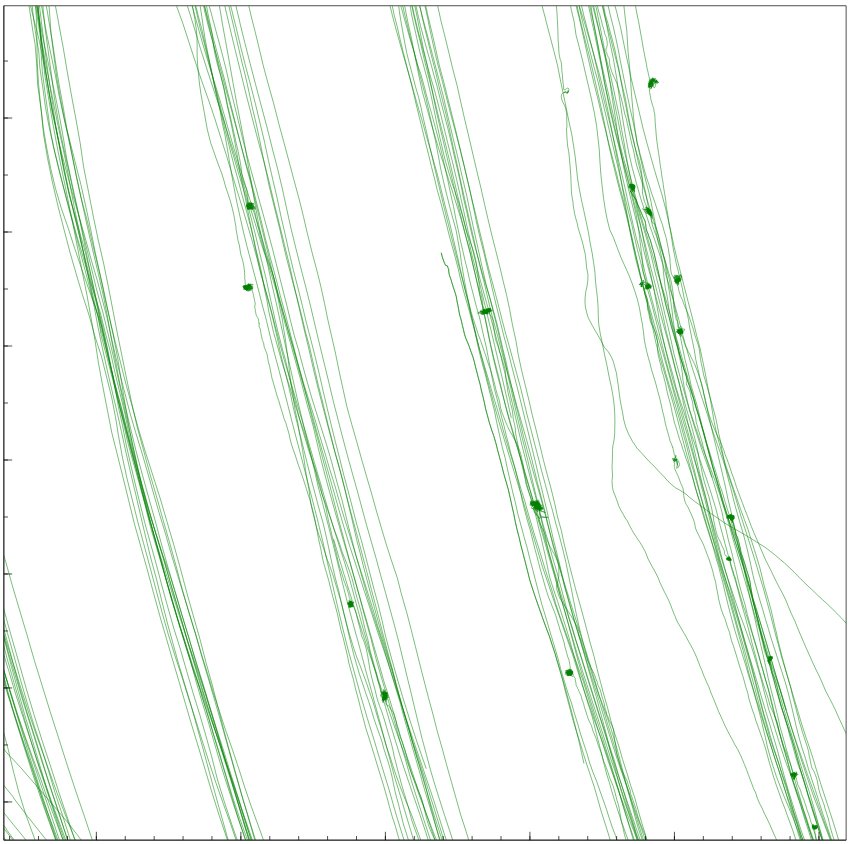
\includegraphics[align=c, width=0.35\linewidth]{../resources/img/umsetzung/U1/trajectories_defect1}
    }}
    \qquad
    \subfloat[]{{
        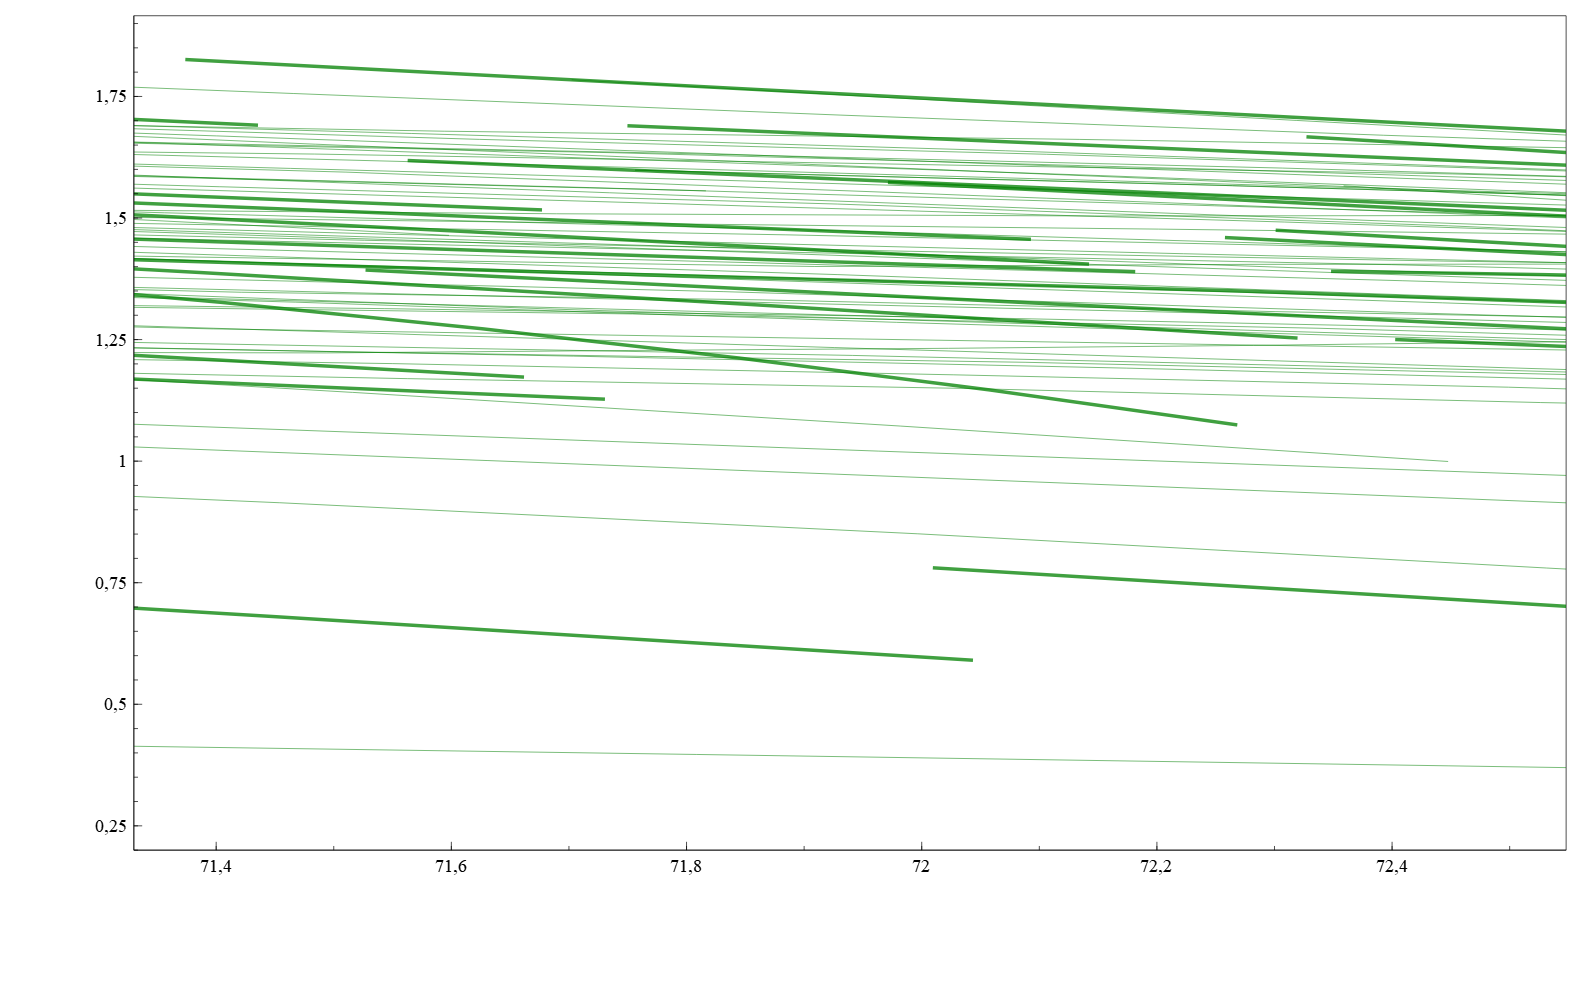
\includegraphics[align=c, width=0.45\linewidth]{../resources/img/umsetzung/U1/trajectories_defect2}
    }}
    \caption{a) Punktwolken vor Lichtsignalanlagen, b) Unterbrechungen aufgrund von Überdeckung}
    \label{fig:real_defects_trajectories}
\end{figure}

Um von diesen und weiteren Effekten bei der Clusteranalyse nicht beeinflusst zu werden, durchlaufen die
``Roh-Trajektorien'' einen Vorverarbeitungsschritt. Dieser wird im nächsten Abschnitt vorgestellt.

\section{Vorverarbeitung der Trajektorien}
\label{sec:realisation_preprocessing}

Die verschiedenen Schritte, welche zur Vorverarbeitung und Bereinigung der Roh-Trajektorien angewandt werden,
sind in diesem Abschnitt geschildert.

Das primäre Ziel der Vorverarbeitung ist es, Ausreißer aus der
Trajektorie-Menge zu entfernen, welche das Ergebnis der Clusteranalyse negativ beeinflussen könnten.
Idealerweise sollen nur jene Trajektorien beibehalten werden, welche eine komplette Bewegung eines
Fahrzeugs auf einem bestimmten Straßenabschnitt repräsentieren. Anhand dieser Trajektorien kann
anschließend die Geometrie der realen Fahrspuren ermittelt werden. Ausreißer wie stehende oder unterbrochene Trajektorien
liefern hingegen keine verwendbaren Informationen für die Spurerkennung.

In nachfolgender Auflistung sind die vier wichtigsten Vorverarbeitungsschritte und ihre Anwendungsreihenfolge
aufgeführt. Die einzelnen Schritte und ihr Hintergrund werden anschließend noch genauer erläutert.

\begin{enumerate}
    \item Resampling von Trajektorien auf minimale Punktdistanz
    \item Entfernung zu kurzer Trajektorien
    \item Entfernung unterbrochener Trajektorien
    \item Anpassung der Trajektorien bei niedrigen Aufnahmewinkeln
\end{enumerate}

\subsection{Resampling von Trajektorien auf minimale Punktdistanz}
Der erste Vorverarbeitungsschritt reduziert die Anzahl der Koordinaten, welche eine Bewegungsbahn beschreiben, erheblich
ohne dabei jedoch wichtige Informationen zu verlieren. Insbesondere dann, wenn sich Fahrzeuge mit niedrigen
Geschwindigkeiten bewegen oder teilweise von Ampeln et cetera. stehen, bestehen die Roh-Trajektorien aus sehr vielen
Punkten, welche oft beinahe identische Positionsinformationen darstellen, das heist nur sehr geringe
Abstände voneinander haben. Für die Beschreibung einer Bewegungsbahn ist diese Punktdichte nicht notwendig
und sogar kontraproduktiv, da sie die Performance der nachfolgenden Schritte stark erhöht. Hiervon ist insbesonders
die Clusteranalyse betroffen.

Aus diesen Gründen werden im ersten Vorverarbeitungsschritt Trajektorien auf eine minimale Punktdistanz
von $0.5\ m$ gebracht. Der hierzu verwendete Algorithmus ist in Listing \ref{lst:pseudo_resampling} dargestellt.
Er verwirft alle aufeinanderfolgende Punkte, welche von einem Referenzpunkt weniger als den geforderten Abstand haben.

\begin{lstlisting}[caption=Pseudocode Trajektorie Resampling, language=FSharp, label=lst:pseudo_resampling]
algorithm resampleTrajectory:
  input:  lastRefPoint
          newTrajPoints
          oldTrajPoints
  output: resampled trajectory points

  while oldTrajPoints is not empty do:
    nextPoint := Head(oldTrajPoints)
    remPoints := Tail(oldTrajPoints)

    if dist(lastRefPoint, nextPoint) < 0.5:
      resampleTrajectory(lastRefPoint, newTrajPoints, remPoints)
    else:
      resampleTrajectory(nextPoint, newTrajPoint ++ nextPoint, remPoints)

  return newTrajPoints
\end{lstlisting}

Nach Anwendung des Algorithmus ist im Fall der Neckartor Aufnahme die durchschnittliche Punktlänge
der Trajektorien von 1094 Koordinaten auf 160 gesunken. Die realen Längen der Bewegungsbahnen bleiben
hingegen nahezu gleich. Die Punktwolken, welche stehende Fahrzeuge erzeugen, werden mittels dieses
Schritts ebenfalls entfernt (siehe Abb. \ref{fig:real_result_2nd_Prepro} b)).


\subsection{Entfernung zu kurzer Trajektorien}
Der zweite Verarbeitungsschritt ist sehr einfach aber dennoch sehr effektiv, da mit seiner Hilfe viele
Trajektorien von beispielsweise stehenden Fahrzeugen oder kurz auftretende Tracking-Fehler entfernt
werden können. Hierzu werden die Längen aller Trajektorien überprüft und jene entfernt, welche
unter bestimmten Grenzwerten liegen. Die hierzu verwendete boolesche Überprüfung ist in Gleichung 
\ref{eq_isShortTrajectory} gegeben. Die Grenzwerte würden experimentell bestimmt und lieferten für die
Testaufnahmen gute Ergebnisse.

\begin{ceqn}
\begin{align}
\label{eq_isShortTrajectory}
    isShortTrajectory(t) =
    \begin{cases}
        1 & \text{if } t.pointLength < 50 \lor t.realLength < 10.0 \\
        0 & \text{otherwise}
    \end{cases}
\end{align}
\end{ceqn}

Das Ergebnis der ersten beiden Vorverarbeitungsschritte ist in Abbildung \ref{fig:real_result_2nd_Prepro} dargestellt.
Die Trajektorien stehender Fahrzeuge, sowie die Punktwolken vor Lichtsignalanlagen und weitere Defekte aufgrund
kleiner Tracking-Fehler wurden entfernt. 

\begin{figure}[H]
    \centering
    \subfloat[]{{
        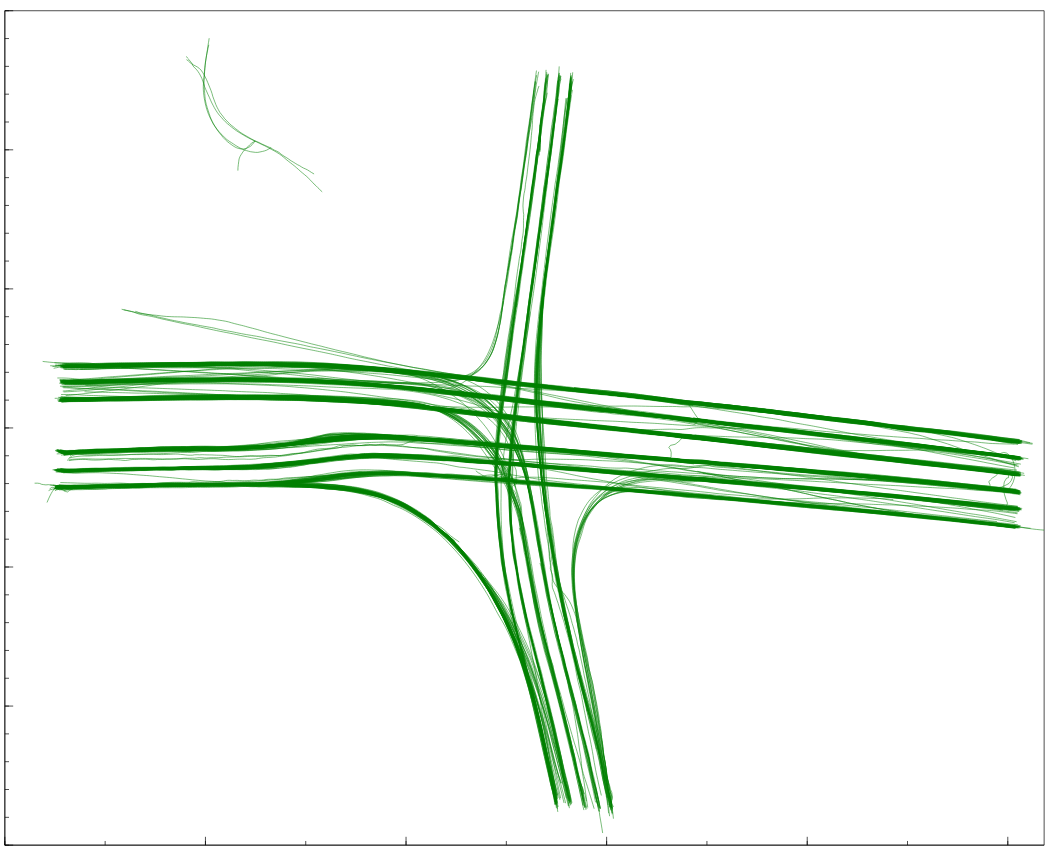
\includegraphics[align=c, width=0.41\linewidth]{../resources/img/umsetzung/U1/trajectories_resampledFiltered}
    }}
    \qquad
    \subfloat[]{{
        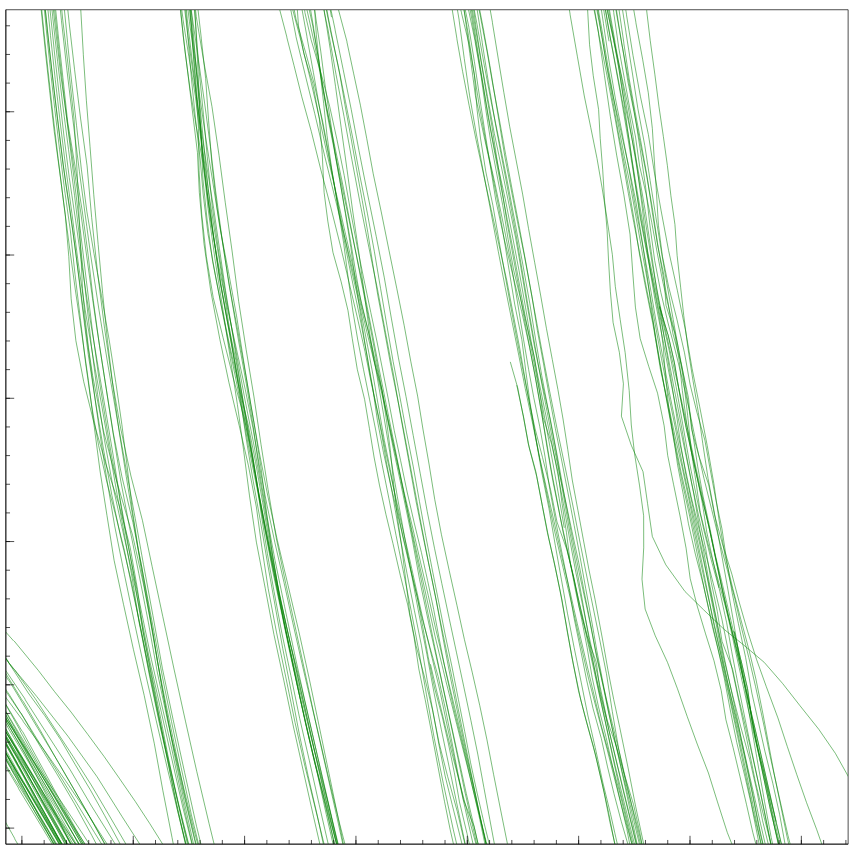
\includegraphics[align=c, width=0.34\linewidth]{../resources/img/umsetzung/U1/trajectories_resampled_cleared}
    }}
    \caption{Ergebnisse der zwei ersten Vorverarbeitungsschritte}
    \label{fig:real_result_2nd_Prepro}
\end{figure}

\subsection{Entfernung unterbrochener Trajektorien}

Nachdem die ersten beiden Verarbeitungsschritte bereits stehende Trajektorien entfernt haben,
müssen nun noch unterbrochene Verfolgungen ausgefiltert werden. Hierzu wird angenommen, dass komplette
Bewegungsbahnen immer im Bereich der Szenenränder beginnen und enden. Wurde eine Fahrzeugverfolgung
unterbrochen, so befinden sich die Anfänge beziehungsweise Enden der daraus resultierenden Trajektorien
im Innenbereich der Aufnahme. Diese Trajektorien werden entfernt. Abbildung \ref{fig:real_completeTrajectory_Definition} 
veranschaulicht das Prinzip der Szenen Rand- und Innenbereiche.

\begin{figure}[H]
\centering
    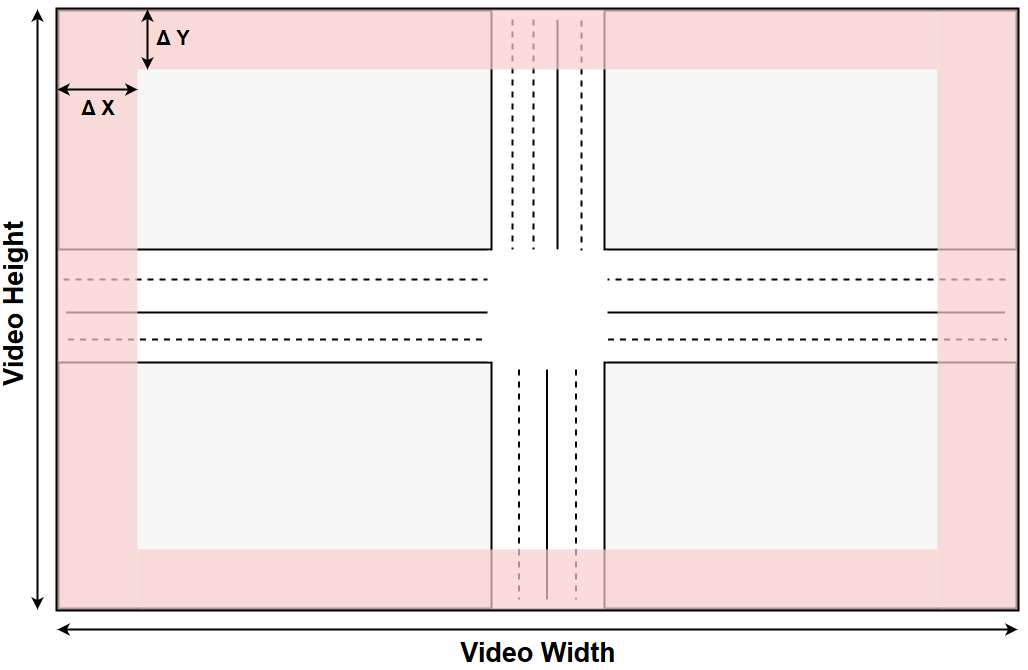
\includegraphics[width=0.5\linewidth]{../resources/img/umsetzung/U1/LaneTopo_CompleteTra}
\caption{Definition von Szenen Rand- und Innenbereich}
\label{fig:real_completeTrajectory_Definition}
\end{figure}

Die Werte $\Delta X$ und $\Delta Y$ entsprechen 10\% der Video-Breite beziehungsweise Höhe.
Ob sich eine Punkt $p$ innerhalb des Szenenrandes befindet, wird mit Hilfe von Formel \ref{eq_inSceneFringe} überprüft.
Hierbei entsprechen $p.sX$ und $p.sY$ den Bildkoordinaten des Punktes $p$.

\begin{ceqn}
\begin{align}
\label{eq_inSceneFringe}
    inSceneFringe(p) =
    \begin{cases}
        1 & \text{if } (p.sX < \Delta X \lor (p.sX > (vWidth - \Delta X))) \\
          &            \lor\ ((p.sY < \Delta Y) \lor (p.sY > (vHeight - \Delta Y))) \\
        0 & \text{otherwise}
    \end{cases}
\end{align}
\end{ceqn}

Nach Ausführung dieses Filter-Schrittes, besteht die Menge der übrigen Trajektorien grundsätzlich nurnoch
aus kompletten Bewegungsbahnen.

Dieser Vorverarbeitungsschritt beruht auf der Annahme, dass für eine Fahrspur neben unterbrochenen auch
ununterbrochene Trajektorien vorliegen, welche eine vollständige Bewegung auf der Spur beschreiben.
Sind alle Trajektorien einer Fahrspur aufgrund einer Verdeckung in der Aufnahme unterbrochen, werden
diese durch das Verfahren vollständig entfernt und eine Extraktion der Spur ist nicht möglich.

\subsection{Anpassung der Trajektorien bei niedrigen Aufnahmewinkeln}


% Endnotes:
%   Problematisch auch Spurwechsel. Hier schwer auszufiltern, da sie Ausreißer in Bezug auf eine Spur darstellen
%   und nicht generelle Ausreißer

\section{Clustering der Trajektorien}
\label{sec:realisation_clustering}

% genaue Beschreibung des Vorgehens, bis finale Clustering Lösung erreicht wurde
% Ansätze: Gründe, Stärken, tatsächliche Problem
% Ansatz A:
%   Mod. Hausdorff Distanz und Spectral Clustering (bas. auf Avet et al.) (Erklärung Grundfunktionsweise Spectral-Clustering)
%   Weil: SC performant, deterministisch, oft verwendet
%   Probleme: Clusteranzahl Bestimmung, Umgehen mit Ausreißern, Tatsächliche Ergebnisse nicht gut
%   --> Performance / Qualität des Ansatzes konnte für vorhandene Daten nicht bestätigt werden
%   --> Problematisch auch Umgang mit vielen Parametern
% Ansatz B:
%   LCSS Distanz (in anderen Papern gute Ergebnisse) (impl. mittels bottom up dyna. programmierung, Verwendung Eucl. Dist.)
%   Wieso D2 aus Vlachos et al. verwendet? (Verschiebung unerwünscht)
%   DBSCAN Clustering
%   --> DM kann besser mit Ausreißern umgehen und DBSCAN berücksichtigt diese auch
%   bessere Ergebnisse

% Probleme: Erkennung von Abbiegespuren, mit wenig Fahrzeugen und Abbiegevorgängen auf mehrere Spuren
%   Dafür: Weitere Verarbeitung der Clustering Outlier
%   Beschreibung Verfahren (dichte-basiert, suchen von initial Dichten Regionen, Verfolgung bis Ausdünnung)

\chapter{Fahrspur-Bestimmung aus Trajektorie-Clustern}
\label{cha:lane_definition}

% Cluster-Bereinigung: Entfernen von Outliern (Spurwechselvorgänge)
%   Beschreibung Probleme: Performance, Zuverlässigkeit (initial Distanzbasiert, erweitert Dichtebasiert --> Ähnliche Ergebnisse und Performance)
%   Verfahren mit evtl. besseren Resultaten noch aufwendiger und basierend meist auf selben Ideen (Distanzmaße, Dichten etc.)
% Bestimmung Referenz-Trajektorie
% Bestimmung von Spur-Envelopes
% Partitionierung der initialen Spur-Schätzungen
% Alignment der Spuren